%!TEX root = ../terrainbook.tex

\graphicspath{{bathymetry/}}

\chapter{Processing bathymetric data to produce hydrographic charts}
\label{chap:bathymetry}

\begin{figure}[ht]
  \centering
  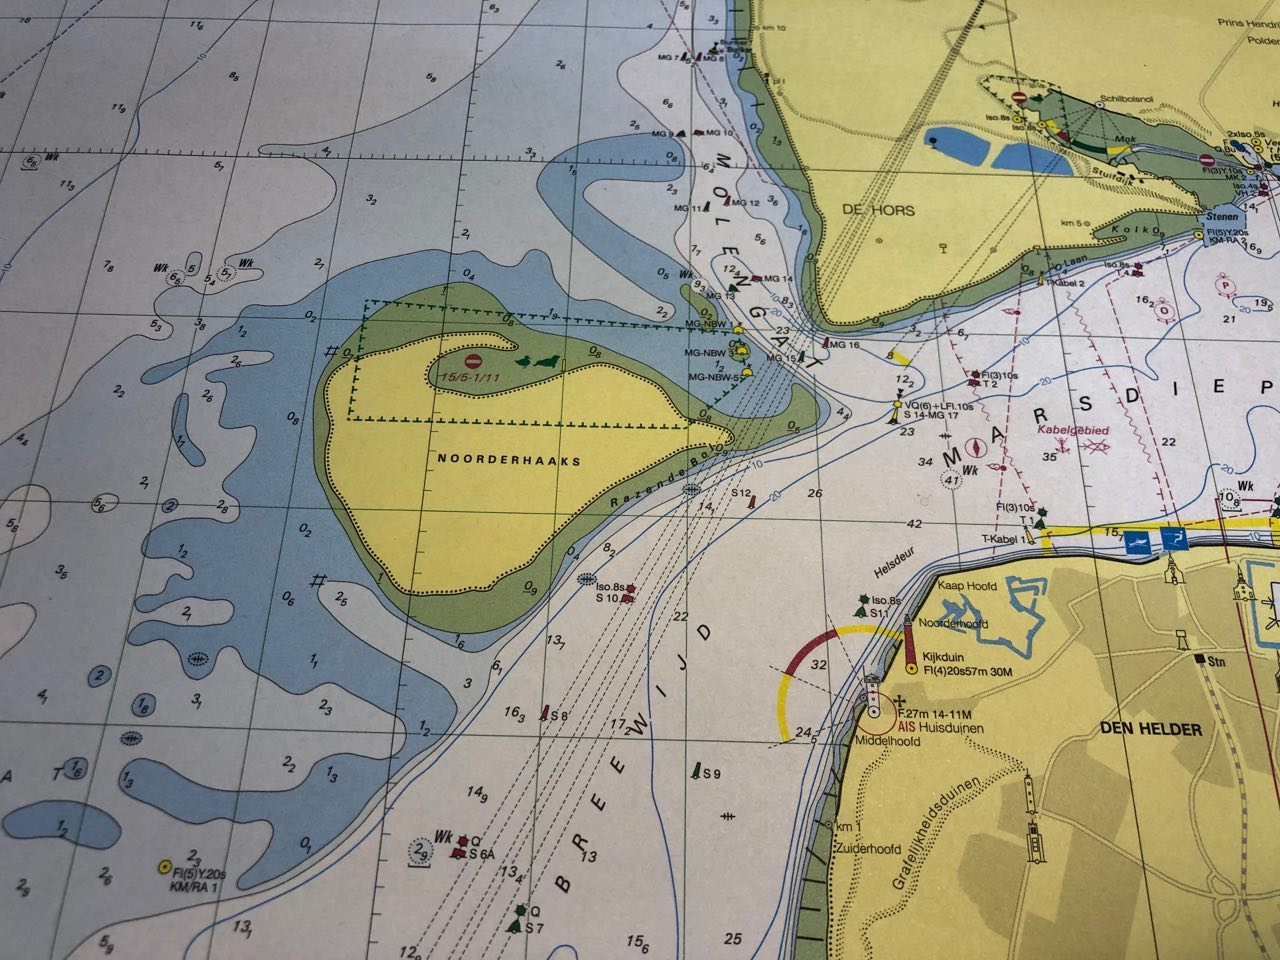
\includegraphics[width=0.8\linewidth]{figs/enc_denhelder.jpeg}
  \caption{An example of an ENC (electronic navigational chart) in the Netherlands. [photo of a paper map from the \emph{Hydrografische Dienst}]}
\label{fig:enc.jpg}
\end{figure}

An hydrographic chart is a map of the underwater world specifically intended for the safe navigation of ships.
In its digital form, it is often called an electronic navigational chart, or ENC.
The information appearing on an ENC are standardised, and there are open formats.

%

We focus in this chapter on one element of these charts: depth-contours, which are akin to isocontours, as seen in Chapter~\ref{chap:conversion}, but show the depth with respect to a given level of water.


%%%
%
\section{How are depth-contours produced in practice?}

Traditionally, the depth-contours have been drawn by hand by skilled hydrographers.
They used a limited set of scattered surveyed depth measurements to deduct and depict the morphology of the seafloor with smooth-looking curves.

%

Nowadays, with technologies such as multibeam echosounders (MBES) offering an almost full coverage of the seafloor (see Section~\ref{sec:mbes}), one would expect the contouring process to be fully automatic.
It is however in practice still a (semi-)manual process since the new technologies have ironically brought new problems: computers have problems processing the massive amount of data, especially in choosing which data is relevant and which is not.

%

Contours constructed directly from MBES datasets are often not satisfactory for navigational purposes since, as Figure~\ref{fig:raw} shows,
\begin{figure}
  \centering
  \begin{subfigure}[b]{0.45\linewidth}
    \centering
    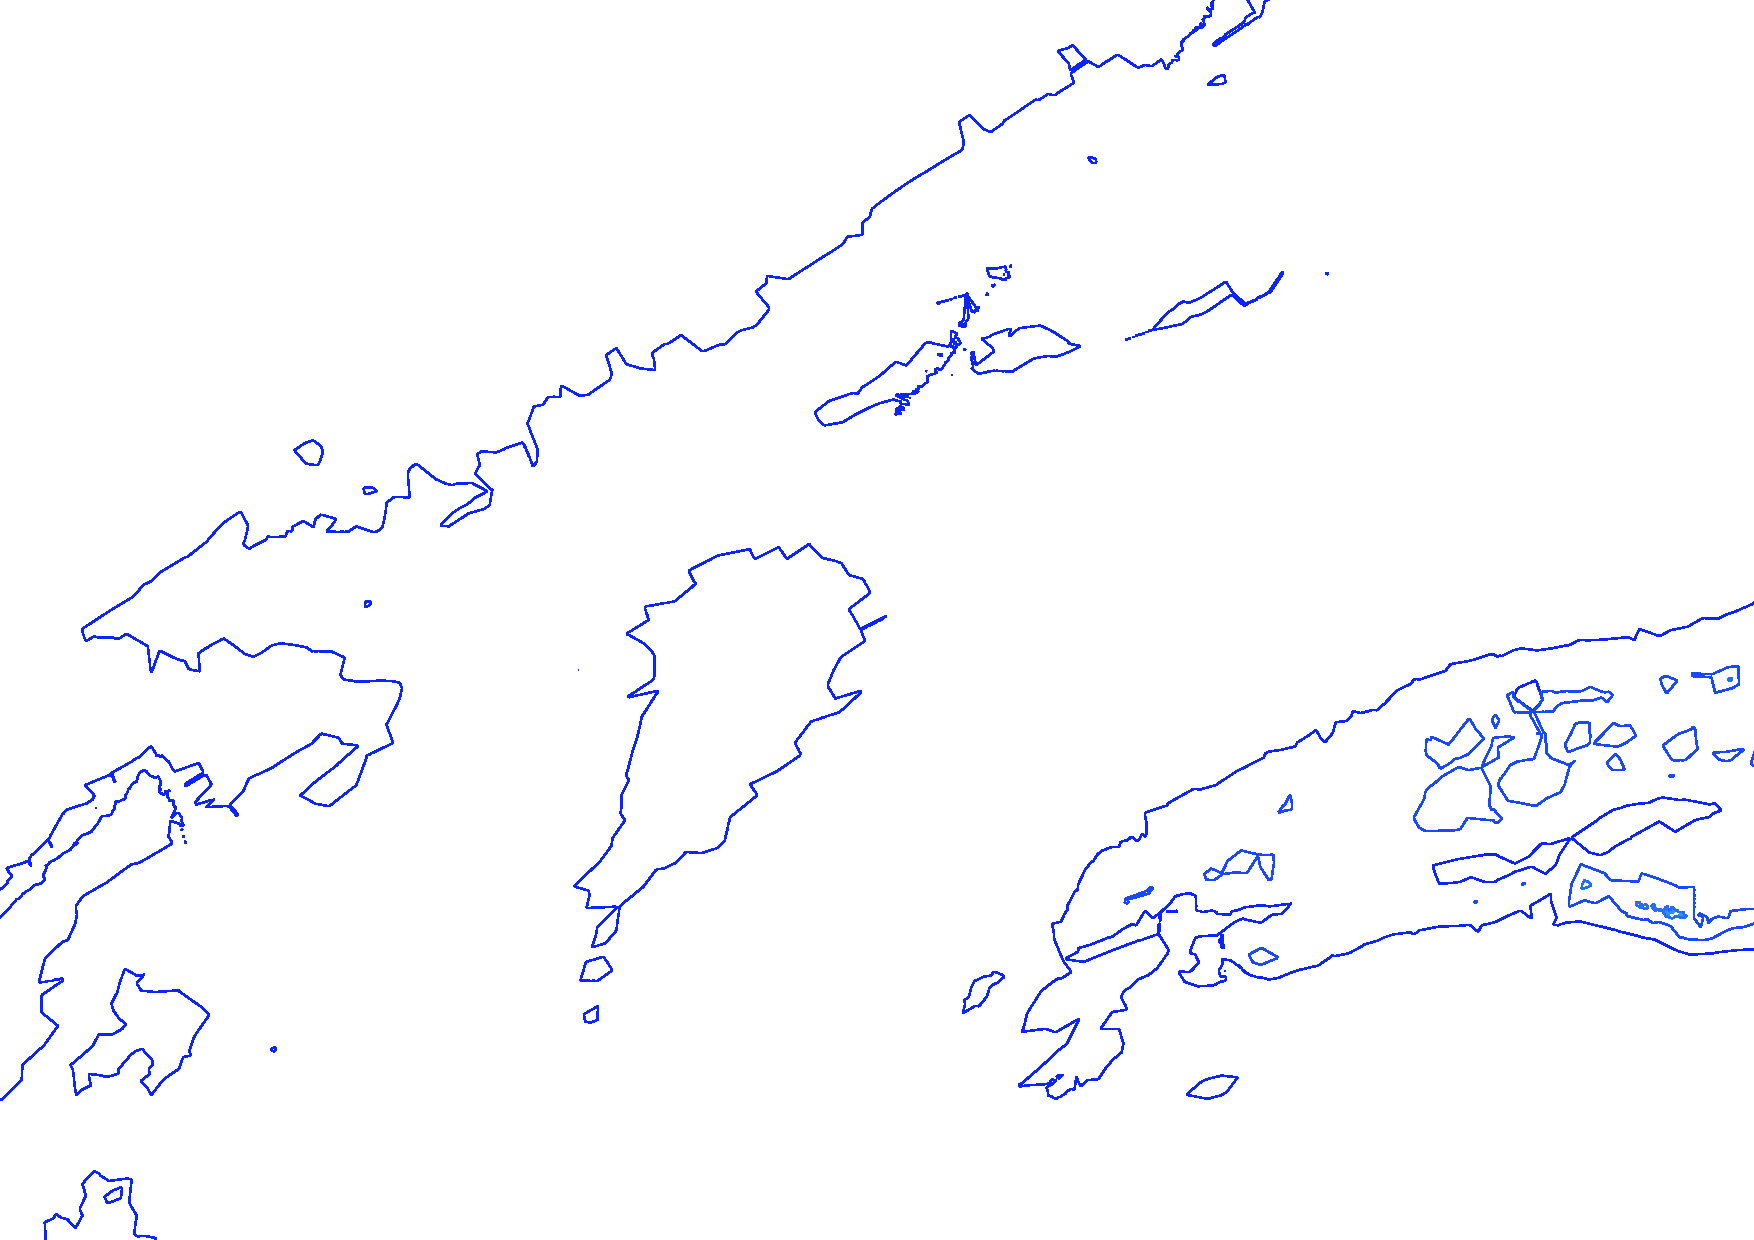
\includegraphics[width=\textwidth]{figs/raw.pdf}
    \caption{}\label{fig:raw}
  \end{subfigure}%
  \begin{subfigure}[b]{0.45\linewidth}
    \centering
    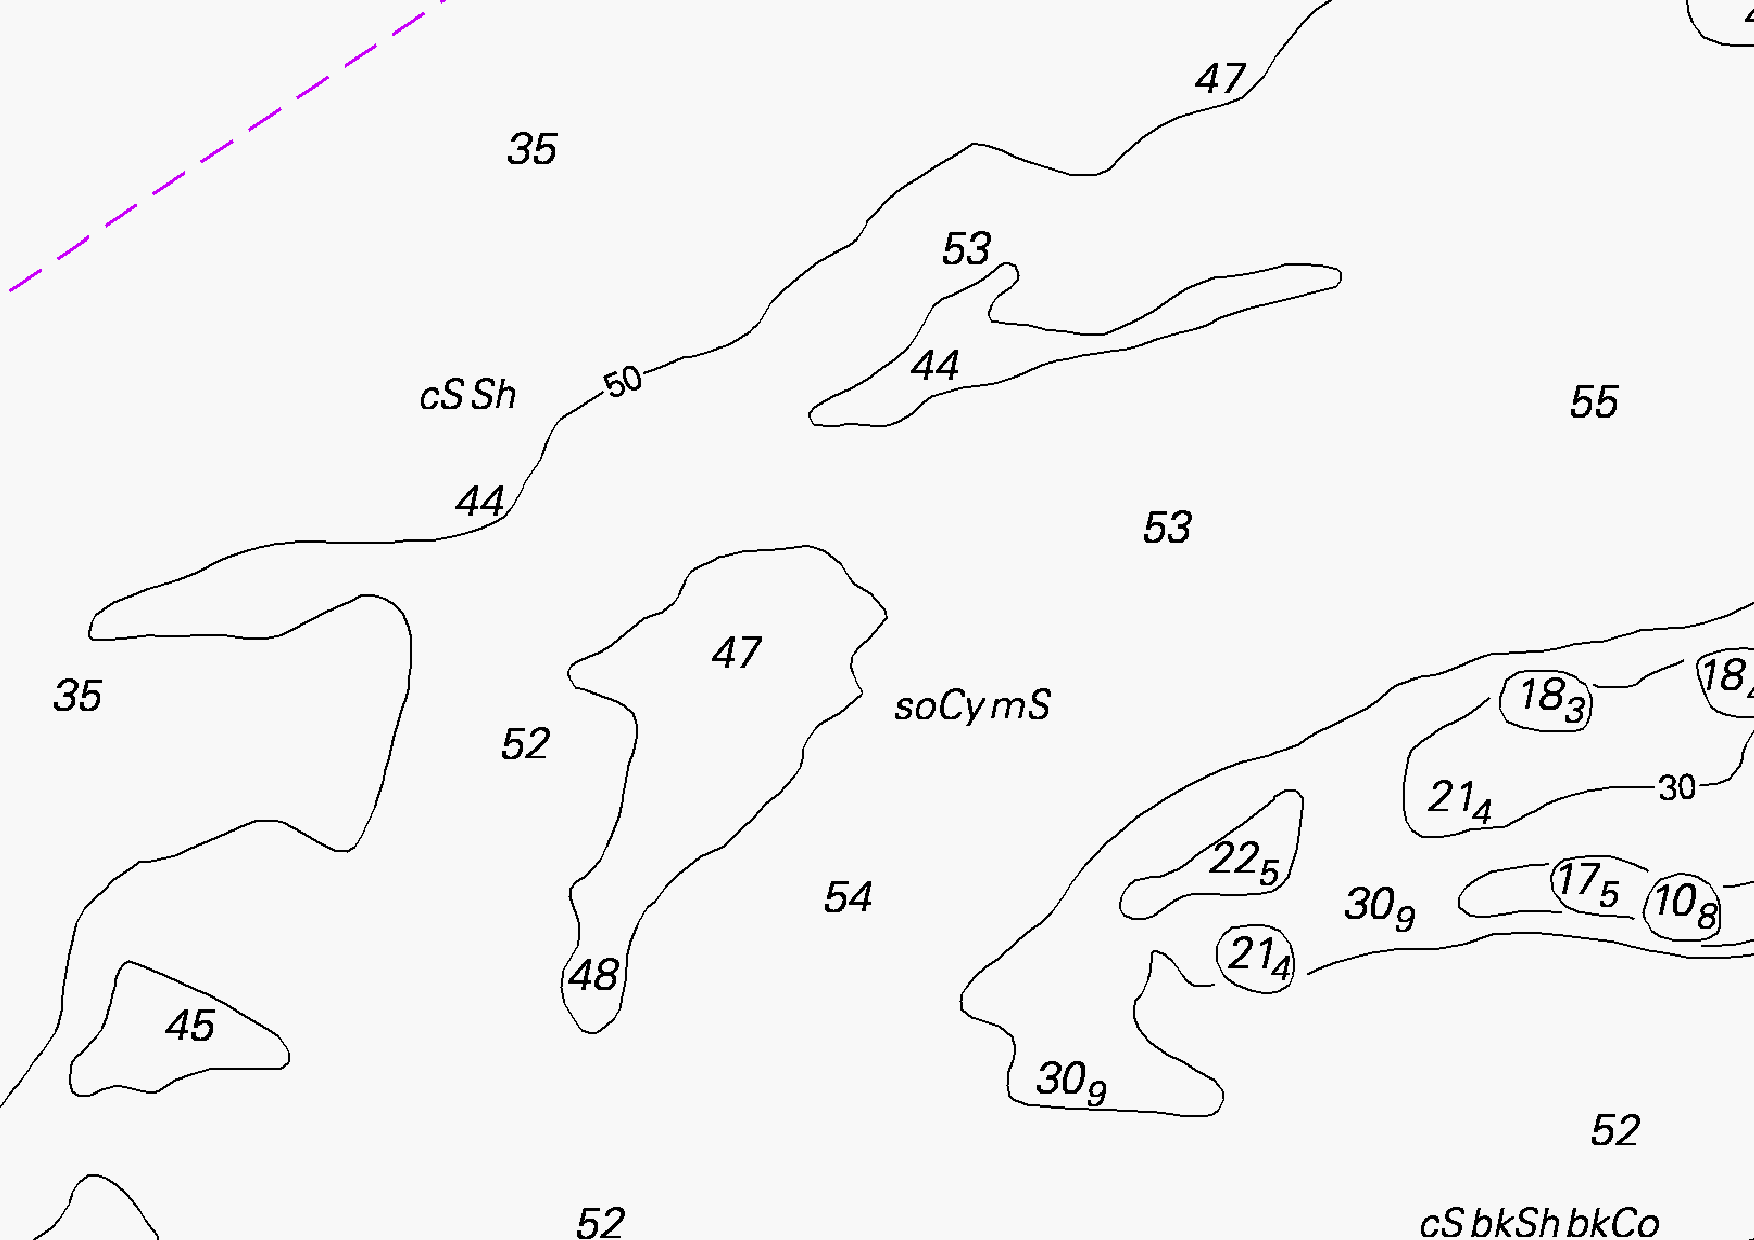
\includegraphics[width=\textwidth]{figs/maponly.pdf}
    \caption{}\label{fig:ideal}
  \end{subfigure}
  \begin{subfigure}[b]{0.45\linewidth}
    \centering
    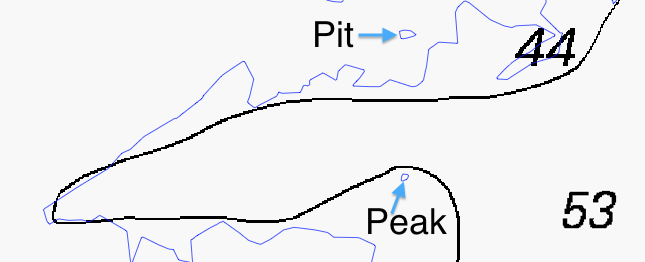
\includegraphics[width=\textwidth]{figs/smoothinAndOmission.png}
    \caption{}
  \end{subfigure}
  \begin{subfigure}[b]{0.45\linewidth}
    \centering
    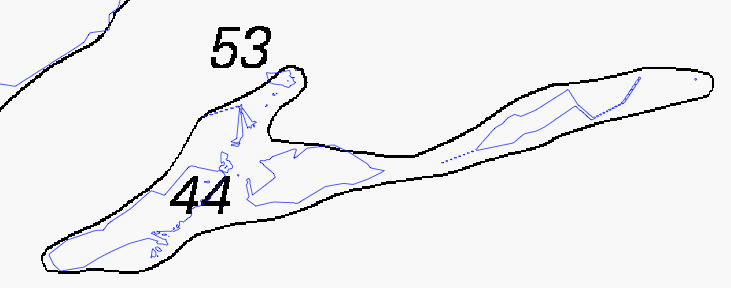
\includegraphics[width=\textwidth]{figs/aggregation.png}
    \caption{}
  \end{subfigure}
\caption{Comparison of \textbf{(a)} depth-contours obtained automatically from the raw MBES data and \textbf{(b)} the hydrographic chart from the Royal Australian Navy for the Torres Strait north of Australia. Raw depth contours are blue, generalized depth contours are black. \textbf{(c)} Pits are removed, while peaks are preserved or integrated with another contour. \textbf{(d)} Groups of nearby contour lines are aggregated}
\label{fig:contouringaspects}
\end{figure}
they are zigzagging (the representation of the seafloor contains ``waves'', \ie\ the slope changes abruptly) and they contain many ``island'' contours (seafloor has several local minima and maxima). 
These artefacts are the result of measurement noise that is present in MBES datasets, \ie\ the variation in depth between two close samples can be larger than in reality, even after the dataset has been statistically cleaned.
Figure~\ref{fig:ideal} illustrates what is expected by hydrographers.


%%%%%%%%%%%%%%%%%%%%
%
\subsection{Generalisation is required to obtain good depth contours}

Creating good depth-contours requires \emph{generalisation}, \ie\ the process of meaningfully reducing information.

%

However, the generalisation of the content of a hydrographic chart is hindered by the fact that four constraints must be respected:
\begin{enumerate}
  \item The \emph{safety constraint}.  
  At every location, the indicated depth must not be deeper than the depth that was originally measured at that location; this is to guarantee that a ship never runs aground because of a faulty map.
  This constraint is a so-called hard constraint, \ie\ it can never be broken.
  \item The \emph{legibility constraint}. 
  An overdose of information slows down the map reading process for the mariner, thus only the essential information should be depicted on the map in a form that is clearly and efficiently apprehensible. %This requires cartographic generalisation.
  \item The \emph{topology constraint}. 
  The topology of the depicted map elements must be correct, \ie\ isocontours may not touch or intersect (also a hard constraint).
  \item The \emph{morphology constraint}. 
  The map should be as realistic and accurate as possible, \ie\ the overall shape of the morphology of the underwater surface should be clearly perceivable and defined features should be preserved.
\end{enumerate}

It should be noted that these four constraints are sometimes incompatible with each other. 
For instance, the morphology constraint tells us to stay close to the measured shape of the seafloor, while the legibility constraint forces us to deviate from that exact shape by disregarding details. 

%

Also, because of the safety constraint, isocontours can only be modified such that the safety is respected at all times: contours can only be pushed towards the deeper side during generalisation, as illustrated in Fig~\ref{fig:genvalidornot}. 
\begin{figure}
  \centering
  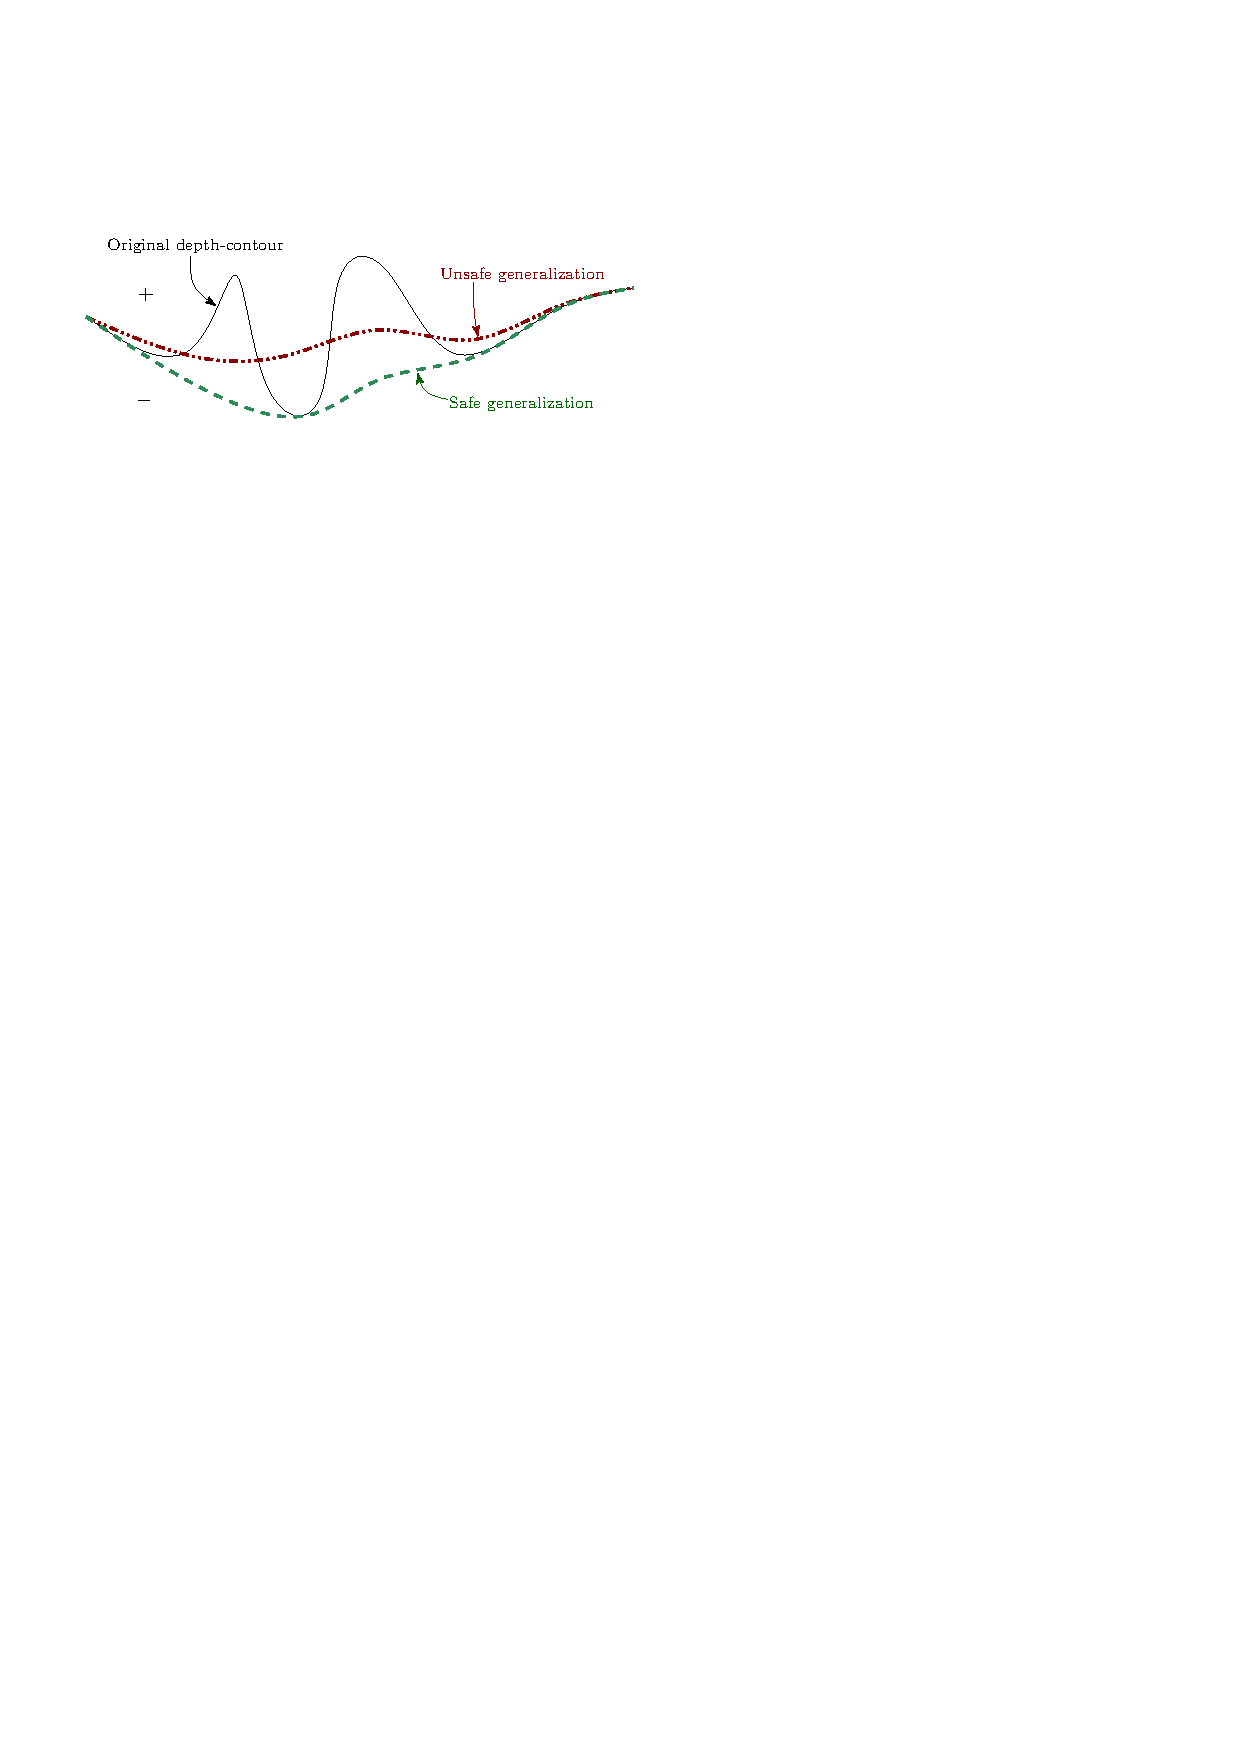
\includegraphics[width=0.5\textwidth]{figs/genvalidornot}
  \caption{During generalisation, depth-contours can only be moved towards greater depth (indicated by a ``--'' in the figure).}
\label{fig:genvalidornot}
\end{figure}
It is therefore evident that the end result must be a reasonable compromise between the four constraints, although the hard constraints must not be broken.


%%%
\section{Common methods used in practice are not satisfactory}

The generation of depth contours, and their generalisation, can be done by several methods.
We present here the most used methodologies.

% We demonstrate in the next section that such workflows can \emph{not} guarantee that the safety constraint is respected, and should therefore not be used.
% This is one result of this paper.

%%%
\subsection{Displacement and generalisation of the lines}

%%%
\subsection{Creation of a simplified raster}

Practitioners usually first interpolate the original MBES samples to create a grid and then directly extract the contours from the grid.
If the number of samples is too high to be processed by a computer, they often use a subset, which has the added benefits of creating smoother and simpler depth-contours.

%%%
\subsection{TIN simplification}



An alternative approach is to construct depth-contours and directly displace the lines.
\citet{Guilbert07} and \citet{Guilbert08} provide the only known methodology to generalise these while respecting the four constraints.
However, these methods require input datasets that are already relatively clean and structured according to a specific format (\emph{b-splines}), and they do not consider how to safely obtain these in the first place.









%%%%%%%%%%%%%%%%%%%%
%
\section{Notes \& comments}

As \citet{Zhang11} state, the generalisation of the content of a nautical chart is hindered by the fact that the following four constraints must be respected:



%%%%%%%%%%%%%%%%%%%%
%
\section{Exercises}

\begin{enumerate}
  \item Bacon ipsum dolour sit amet porchetta beef turkey, bacon turducken boudin hamburger venison ball tip. Brisket pork loin bresaola short loin ground round leberkas pastrami tongue jerky cow turducken beef ribs. Pork ribeye landjaeger prosciutto pig venison tenderloin. Swine beef ribs kielbasa, porchetta tenderloin salami venison pork belly tail.
  \item Bacon ipsum dolour sit amet porchetta beef turkey, bacon turducken boudin hamburger venison ball tip. Brisket pork loin bresaola short loin ground round leberkas pastrami tongue jerky cow turducken beef ribs. Pork ribeye landjaeger prosciutto pig venison tenderloin. Swine beef ribs kielbasa, porchetta tenderloin salami venison pork belly tail.
\end{enumerate}